\documentclass[12pt]{beamer}
\usepackage{cmap}
\usepackage[T2A]{fontenc}
\usepackage[utf8]{inputenc}
\usepackage{ifluatex}
\usefonttheme[onlymath]{serif}
\usepackage{svg}
\usepackage{enumerate}
\usepackage{hyperref}
\usepackage{mathtools}
\setbeamertemplate{footline}[frame number]
\definecolor{beamer@darkgreen}{rgb}{0,0.6,0}
\setbeamercolor{normal text}{fg=black,bg=white}
\setbeamercolor{title}{fg=black,bg=beamer@darkgreen}
\setbeamercolor{frametitle}{fg=black,bg=beamer@darkgreen}
\setbeamercolor{background canvas}{parent=normal text}

\usepackage[english,russian]{babel}
\usepackage{graphicx}
\usepackage{listings}
\DeclareMathOperator{\sign}{sign}

\usepackage{enumerate}

\author{Катя Тузова}
\title{Машинное обучение}
\date{}

\subtitle{Лекция 1}

\begin{document}
\frame{\titlepage}

\begin{frame}\frametitle{Правила игры}
\begin{itemize}
  \item[--] 13 опросов по 5 баллов в начале лекции
  \item[--] 13 домашних заданий по 20 баллов при сдаче в первую неделю, 
  10 баллов при сдаче во вторую неделю
  \item[--] 1 соревнование на платформе kaggle.com - 40 баллов
  \vspace{5mm}
  \item[--] Допуск к экзамену = 150 баллов
  \item[--] Экзамен = 3 вопроса
  \item[--] За каждые 70 баллов сверх 150 -- минус вопрос на экзамене
\end{itemize}
\end{frame}

\begin{frame}\frametitle{Что такое машинное обучение?}
\end{frame}

\begin{frame}\frametitle{Что такое машинное обучение?}
(Wikipedia)\\
Machine learning is a scientific discipline that explores the construction and study of algorithms that can learn from data. Such algorithms operate by building a model based on inputs and using that to make predictions or decisions, rather than following only explicitly programmed instructions. 
\vspace{5mm}

Обширный подраздел искусственного интеллекта, изучающий методы построения моделей, способных обучаться, и алгоритмов для их построения и обучения.\\

\end{frame}

\begin{frame}\frametitle{В чем отличия ML от AI?}
\end{frame}

\begin{frame}\frametitle{Разделы AI}
\begin{itemize}
  \item[--] Работа с естественными языками
\item[--] Представление и использование знаний
\item[--] Компьютерное зрение
\item[--] Машинное обучение
\item[--] Биологическое моделирование искусственного интеллекта
\item[--] Робототехника
\item[--] Анализ графов
\item[--] \ldots
\end{itemize}
\end{frame}

\begin{frame}\frametitle{Что такое машинное обучение?}
Arthur Samuel (1959). \\
\vspace{5mm}
Field of study that gives computers the ability to learn without being explicitly programmed.
\end{frame}

\begin{frame}\frametitle{Пример}
Чем отличается задача “найти кратчайший путь в графе” от “антиспам фильтр”?
\end{frame}

\begin{frame}\frametitle{Что такое машинное обучение?}
Tom Mitchell (1998) \\
\vspace{5mm}
Well-posed Learning Problem: A computer program is said to learn from experience E with respect to some task T and some performance measure P, if its performance on T, as measured by P, improves with experience E\\
\vspace{5mm}
E.g., Learn to play checkers\\ 
\vspace{5mm}
T : Play checkers\\
P : \% of games won in world tournament\\
E : opportunity to play against self\\
\end{frame}

\begin{frame}\frametitle{Где используется ML?}

\end{frame}

\begin{frame}\frametitle{Где используется ML?}
\begin{itemize}
  \item[--] Рекомендации на Amazon, Kinopoisk
  \item[--] Поисковые системы Google, Яндекс
  \item[--] Выделение лиц друзей на фото Facebook
  \item[--] Боты в Twitter
\end{itemize}
\end{frame}

\begin{frame}\frametitle{Какая математика понадобится?}

\end{frame}

\begin{frame}\frametitle{Какая математика понадобится?}
\begin{itemize}
  \item[--] Математическая статистика 
  \item[--] Методы оптимизации 
  \item[--] Дискретная математика
  \item[--] Теория вероятности
  \item[--] Линейная алгебра
\end{itemize}
\end{frame}

\begin{frame}\frametitle{Вопрос}
Кто из вас уже использовал методы машинного обучения? 
\end{frame}

\begin{frame}\frametitle{Метод наименьших квадратов}
\begin{figure}[htbp]
  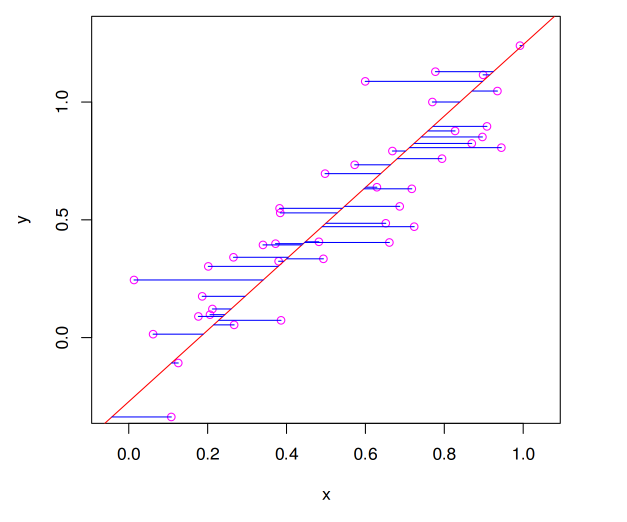
\includegraphics[height=100pt, keepaspectratio = true]{OLS1}  
  \hspace{30px}
  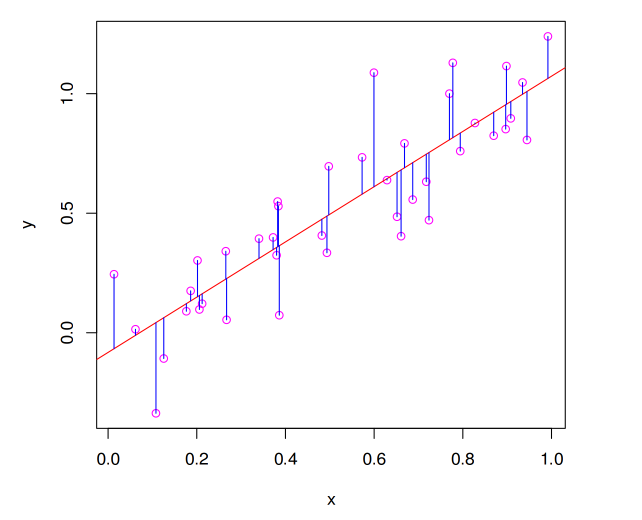
\includegraphics[height=100pt, keepaspectratio = true]{OLS2}  
  \hspace{30px}
  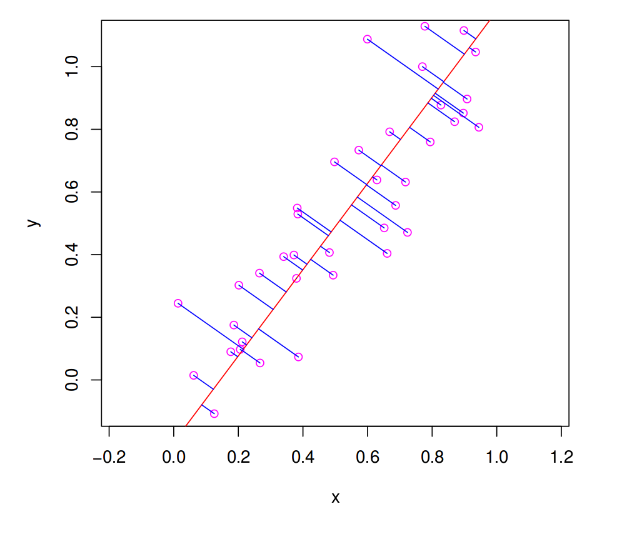
\includegraphics[height=100pt, keepaspectratio = true]{OLS3}  
\end{figure}
\end{frame}

\begin{frame}\frametitle{Метод наименьших квадратов}
Идея: Аппроксимировать данные линейной зависимостью \\
Суть: Минимизация суммы квадратов отклонений данных от прямой\\
\end{frame}

\begin{frame}\frametitle{Вопрос}
    Достаточно ли знать алгоритмы ML и математику?
\end{frame}

\begin{frame}\frametitle{Что еще надо понимать}

\begin{itemize}
  \item[--] Когда надо применять ML
  \item[--] Как сформулировать задачу в терминах ML
  \item[--] Как выбрать подходящий класс алгоритмов
  \item[--] Где посмотреть существующие решения
  \item[--] Как настроить алгоритм
  \item[--] Как оценить результаты
\end{itemize}
\end{frame}


\begin{frame}\frametitle{Тест Тьюринга}
    AI как наука начался с теста Тьюринга (1950).\\
    \vspace{5mm}
    Компьютер должен успешно выдать себя за человека в (письменном) диалоге между судьёй, человеком и компьютером
\end{frame}

\begin{frame}\frametitle{История ML}
\begin{itemize}
  \item[--] 50-70 гг. -- Базы знаний, полнотекстовый поиск, распознавание образов, нейронные сети, К ближайших соседей.
  \item[--] 1973г. -- “Зима” искуственного интеллекта
  \item[--] 80-90гг.  -- Первые конференции, развитие практического применения
  \item[--] 90-00гг. -- Метод опорных векторов, бустинг
  \item[--] Рандомизированный решающий лес (начало 2000х)
  \item[--] Обучение Марковских случайных полей (2000е)
  \item[--] Глубокое обучение (2006)
\end{itemize}
\end{frame}

\begin{frame}\frametitle{Зима AI}
\begin{itemize}
  \item[--] Проблема комбинаторного взрыва
  \item[--] Низкая производительность компьютеров
  \item[--] Проблема представлений знаний “здравого мысла”
  \item[--] Парадокс Моравеца
\end{itemize}
\end{frame}

\begin{frame}\frametitle{Типы машинного обучения}
\end{frame}

\begin{frame}\frametitle{Типы машинного обучения}
\begin{itemize}
  \item[--] С учителем
  \item[--] Без учителя
  \item[--] Смешанное
\end{itemize}
\end{frame}

\begin{frame}\frametitle{Обучение с учителем (Классификация)}
\begin{figure}[htbp]
\centering
\includesvg[height=200pt]{Classification}  
\end{figure}
\end{frame}

\begin{frame}\frametitle{Обучение с учителем (Регрессия)}
\begin{figure}[htbp]
\centering
\includesvg[height=200pt]{Regression1}  
\end{figure}
\end{frame}

\begin{frame}\frametitle{Обучение с учителем (Регрессия)}
\begin{figure}[htbp]
\centering
\includesvg[height=200pt]{Regression2}  
\end{figure}
\end{frame}

\begin{frame}\frametitle{Обучение с учителем (Регрессия)}
\begin{figure}[htbp]
\centering
\includesvg[height=200pt]{Regression3}  
\end{figure}
\end{frame}


\begin{frame}\frametitle{Обучение с учителем }
Множество объектов $X$ \\
Множество допустимых ответов $Y$\\
Прецедент - пара объект-ответ ${(x_i,y_i)}$  \\
Обучающая выборка - совокупность пар ${X_l = (x_i,y_i)_{i=1}^l}$ \\
Целевая функция ${y^*:X \rightarrow Y}$\\
\vspace{5mm}
Задача обучения по прецедентам:\\
Найти решающую функцию ${a: X \rightarrow Y}$  \\
Решающая функция должна приближать целевую на всем множестве ${X}$
\end{frame}

\begin{frame}\frametitle{Пример. Метод наименьших квадратов}
Линейная модель:\\
${y(x, w) = \sum\limits_{i=1}^l x_i w_i }$ \\
\vspace{5mm}
Целевая функция?\\
\vspace{5mm}
Решающая функция?
\end{frame}

\begin{frame}\frametitle{Пример. Метод наименьших квадратов}
Линейная модель:\\
${y(x, w) = \sum\limits_{i=1}^l x_i w_i }$ \\
Целевая функция:
${y^* = \sum\limits_{i=1}^l (y_i - y(x, w))^2}$ \\
\vspace{5mm}
Решающая функция - итог оптимизации:
${\arg\min_w y^*}$
\end{frame}

\begin{frame}\frametitle{Обучение с учителем }
\begin{itemize}
  \item[--] Классификация (${Y={1,2,..,K}}$ конечно) — множество $X$ разбивается на $K$ классов. Требуется предсказать к какому классу он принадлежит. 
  \item[--] Восстановление регрессии ${(Y=\mathbb{R})}$ — требуется найти функцию $f$ из определенного класса, которая аппроксимирует $f^*$
\end{itemize}
\end{frame}

\begin{frame}\frametitle{Обучение без учителя (Пример) }
\begin{figure}[htbp]
\centering
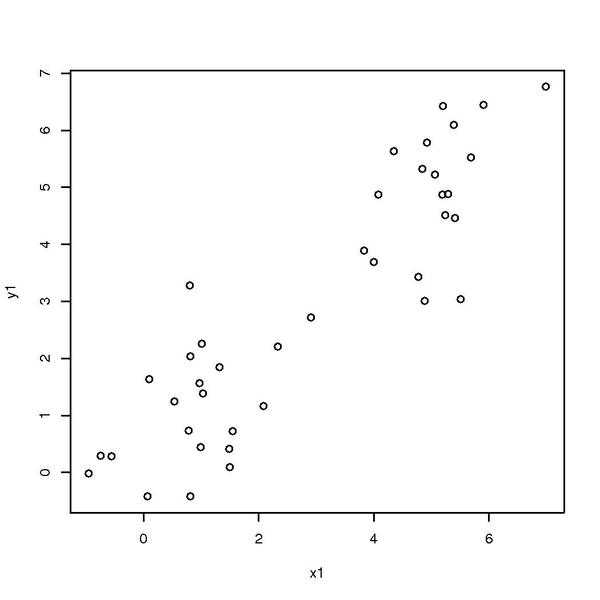
\includegraphics[height=200pt]{Clustering1}  
\end{figure}
\end{frame}

\begin{frame}\frametitle{Обучение без учителя (Пример) }
\begin{figure}[htbp]
\centering
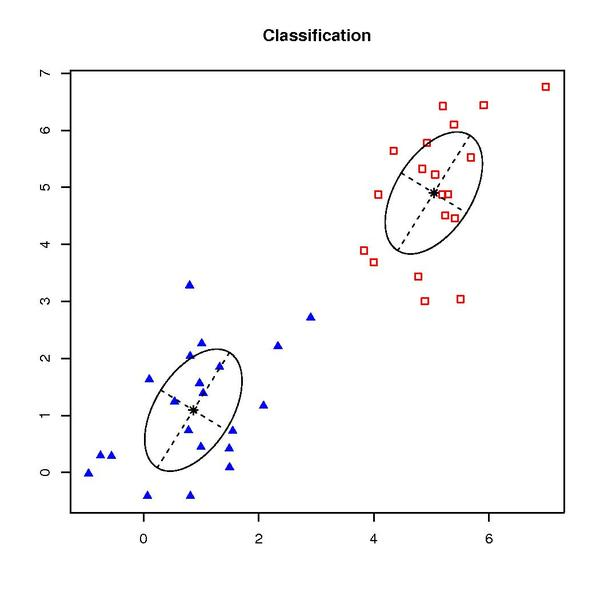
\includegraphics[height=200pt]{Clustering2}  
\end{figure}
\end{frame}

\begin{frame}\frametitle{Типы признаков}
${f: X \rightarrow D_f}$
\begin{itemize}
  \item[--] Бинарные (${D_f = \left\{ 0, 1 \right\} }$)
  \item[--] Номинальные (${D_f}$ -- конечное множество)
  \item[--] Порядковые (${D_f}$ -- конечное упорядоченное множество)
  \item[--] Количественные (${D_f = \mathbb{R} }$)
\end{itemize}
\end{frame}

\begin{frame}\frametitle{Типы признаков (примеры)}
\begin{itemize}
  \item[--] Бинарные (Пол, наличие боли в спине, в сознании ли пациент)
  \item[--] Номинальные (Тип боли: колющая, режущая, ноющая)
  \item[--] Порядковые (Общее состояние больного: удовлетворительное, средней тяжести, тяжелое, крайне тяжелое)
  \item[--] Количественные (Температура тела, пульс, артериальное давление)
\end{itemize}
\end{frame}


\begin{frame}\frametitle{Определения}
Переобучение (overfitting) это явление, при котором алгоритм слишком приспособлен для данных, на которых он обучался. Переобучение имеет место при выборе слишком сложных моделей.\\
\vspace{5mm}
\begin{figure}[htbp]
  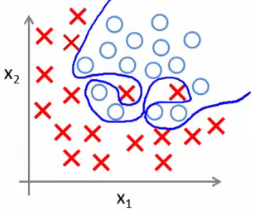
\includegraphics[height=100pt, keepaspectratio = true]{overfitting}  
\end{figure}

\end{frame}


\begin{frame}\frametitle{Определения}
Недообучение (underfitting) это явление, обратное переобучению, при котором алгоритм не полностью использует предоставленные ему для обучения данные. Недообучение имеет место при выборе недостаточно сложных моделей.
\vspace{5mm}
\begin{figure}[htbp]
  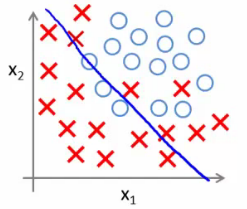
\includegraphics[height=100pt, keepaspectratio = true]{underfitting}  
\end{figure}

\end{frame}

\begin{frame}\frametitle{Применение ML}
\begin{itemize}
  \item[--] Академическое\\
Красивые идеи, хорошая математика
  \item[--] Практическое\\
  Обеспечивает некоторое качество на множестве примеров\\
\end{itemize}
\end{frame}

\begin{frame}\frametitle{Что читать/смотреть}
\begin{itemize}
  \item[--] G. James, D. Witten, T. Hastie, R. Tibshirani: "An Introduction to Statistical Learning" 
  \item[--] Christopher M. Bishop "Pattern Recognition and Machine Learning"
  \item[--] Kevin P. Murphy "Machine Learning A Probabilistic Perspective"
  \vspace{10mm}
  \item[--] К.В. Воронцов. \url{http://shad.yandex.ru/lectures/machine_learning.xml}
  \item[--] Andrew Ng \url{http://ml-class.org/}
\end{itemize}
\end{frame}

\begin{frame}\frametitle{На следующей лекции}
\begin{itemize}
  \item[--] Метод ближайших соседей
  \item[--] Гипотеза компактности
  \item[--] Обобщенный метрический классификатор
  \item[--] Проклятие размерности  
  \item[--] Отбор эталонов    
  \item[--] Автоматический выбор фич  
\end{itemize}
\end{frame}


\end{document}
